\documentclass[12pt,fleqn]{article}\usepackage{../common}
\begin{document}
\textbf{Log Lineer Modeller ve Kosulsal Rasgele Alanlar (Log Linear Models and
Conditional Random Fields -CRF-)}

Ders 2

Charles Elkan ders notlari

Elkan'in makine ogrenimi konusuna bakisi ilginc, ona gore makine ogrenimi
bir bilgisayar bilim (computer science) konusudur, mesela altta islenen
maksimum olurluk bilgisayar bilimdir. 

Kosulsal Olurluk (Conditional Likelihood)

Diyelim ki elimizde egitim verisi olarak ikili $<x,y>$ veri noktalari
var. O zaman $y$'nin $x$'e kosulsal olarak bagli (conditional on) bir
dagilimi oldugunu soyleyebiliriz. 

$$ y \sim f(x;\theta) $$

Yani her $x$ icin farkli bir $y$ dagilimi ortaya cikabilir. Ve tum bu
farkli dagilimlarin ortak noktasi $\theta$ parametresidir. Kosulsal
olasilik yani soyle yazilabilir, 

$$ P(Y=y | X=x;\theta) $$

Usttekiler $Y$ icin bir model ortaya koydu, peki elimizde $X$'in dagilimi
icin bir olasilik modelimiz var mi? Cevap hayir. Niye? Dusunelim, $p(y,x)$
nedir ?

$$ p(x,y) = p(x)p(y|x) $$

Ustte $p(y|x)$'i tanimlayacak ($\theta$ uzerinden) bir olasilik demeti /
ailesi tanimladik, fakat elimizde $p(x)$ dagilimini verecek bir model
yok, o zaman $p(x,y)$'yi tanimlayacak bir model de yok.

Fakat bu dunyanin sonu degil. Belki de Makine Ogrenimi bransinin bir
slogani su olmali: ``Ogrenmen gerekmeyen seyi ogrenme''. Ustteki ornekte
$p(y|x)$'i ogrenebiliriz, ama $p(x)$'i illa ogrenmemiz gerekir mi?

Siniflayici (classifier) ve takip edilen (supervised) ogrenim durumunu
dusunursek, bize egitim amacli olarak $<x,y>$ ikili veri noktalari
saglanacak. $x$ kaynak veri, $y$ tahmin edilecek (ya da basta egitim hedefi
olan) etiket olacak. $y$ icin bir model ortaya cikartiyoruz, cunku test
zamaninda $y$ olmayacak, fakat $x$ hep olacak. Yani $y$'nin modellenmesi
mecburi, cunku ``genelleyerek'' onun ne oldugunu bulacagiz, ama $x$ hep
verili.

Kosulsal Olurluk Maksimum Olurluk Prensibi

Egitim verisi $<x_1,y_1>,...,<x_n,y_n>$ icin, $\theta$'yi soyle sec

$$ \hat{\theta} =  \arg\max_{\theta} \prod _{i=1}^{n} p(y_i | x_i;\theta) $$

Normal maksimum olurlukta bilindigi gibi olasiliklarin carpimi maksimize
edilir, burada maksimize ettigimiz ``kosulsal'' olasiliklarin carpimi. 

Burada onemli bir soru su: bildigimiz gibi maksimum olurluk hesabi her veri
noktasinin bir digerinden bagimsiz oldugunu farzeder [cunku her olurluk
hesabini bir diger ile carpiyoruz, baska ek carpim, toplama, vs
yapmiyoruz], bu faraziye dogru bir faraziye midir? Bu soru ve ona verilecek
cevap cok onemli. Evet, eger egitim noktalari birbirinden bagimsiz degilse
maksimum olurluk kullanmamaliyiz. Bagimsizligi da iyi tanimlamak gerekiyor
tabii, eger ustteki durumda $x_i$ {\em verildikten sonra} $y_i$'larin
birbirinden bagimsiz olmasi yeterli.

Bu model klasik Istatistik'te cokca kullanilan bir yaklasimdir, hatta
lineer regresyon'un temeli ustteki faraziyedir. 

$$ y = \alpha + \bar{\beta}\bar{x} + N(0,\sigma^2) $$

Bu standart lineer regresyon modeli, ve bu modelde her $y$ ona tekabul eden
$x$'e bagli, bu sayede $x$'ler biliniyorsa $y$'ler birbirinden kosulsal
olarak bagimsiz hale geliyor, boylece $x$'ler birbirine bagimli olsa bile
$\alpha$ ve $\beta$'nin bulunmasi mumkun oluyor. 

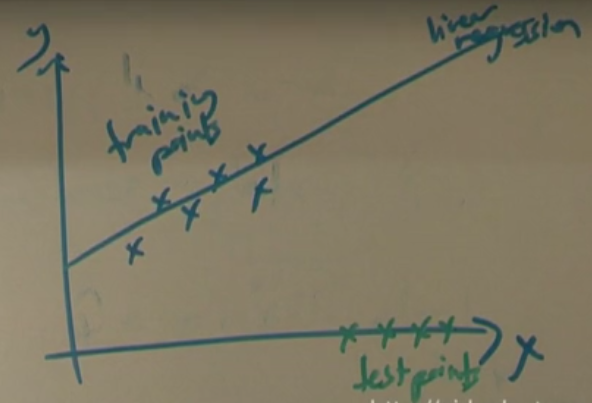
\includegraphics[height=4cm]{crf_1.png}

Ustteki resimde egitim noktalari (training points) mavi olsun, test
noktalari yesil olsun (hemen altinda). Bazi Yapay Ogrenim yaklasimlari
diyebilir ki egitim $x$'lerinin dagilimi test $x$'lerinin dagilimindan
farkli, bu veri seti ogrenilemez (yani genellenemez, modellenemez). Fakat
klasik Istatistik buna bakar ve der ki $x$'lerin verildigi durumda $y$'ler
bagimsizdir, bu sekilde bir kosulsal model ogrenilebilir.

Lojistik Regresyon ayni sekilde isler (lojistik regresyon, log lineer
modellerin ozel bir halidir, CRF'ler ayni sekilde). Burada
da ogrenilen bir

$$ p = p(y | x;\alpha,\beta) $$

modeli vardir ve $y$ degerleri sadece 0 ve 1 olabilir. Tahmin edilen
olasilik ise $y$'nin 1 olma olasiligidir. Bu model Rasgele Gradyan Cikisi
ile egitilir [detaylar icin {\em Lojistik Regresyon} notlarimiza
bakabilirsiniz].

$$ log \frac{p}{1-p} = \alpha + \sum_j \beta_j x_j $$

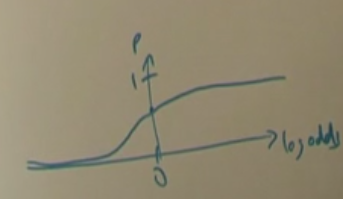
\includegraphics[height=4cm]{crf_2.png}

$p$ log sansinin monotonik bir fonksiyonudur, ve ters yonden bakarsak, log
sans $p$'nin monotonik bir fonksiyonudur. Yani lineer bir fonksiyon (sag
taraf) ne kadar buyurse, olasilik / log sans o kadar buyuyecektir. Bu
buyume durumu mesela $\beta_j$ katsayisini veri analizi baglaminda
yorumlanabilir hale getirir. Diyelim ki $\beta_4$ katsayisi pozitif, o
zaman diger tum sartlarin esit oldugu durumda (with all else being equal)
$x_4$ ne kadar buyurse 1 olma olasiligi o kadar artar.

Lojistik modellerin onemli bazi avantajlari var, ki bu avantajlar log
lineer modellere de sirayet ediyor (bu iyi). 

1) Degiskenler arasi ilinti (correlation) probleme yol acmaz: Bu fayda
aslinda daha once belirttigimiz $x$'lerin birbirine bagimli olabilmesi ile
alakali. Bagimsizlik onsarti aranmadigi icin istedigimiz kadar $x$'i
problemin uzerine atabiliriz, egitici algoritma bunlardan cikartabildigi
kadar iyi bir model bulacaktir.

Kiyasla mesela Naive Bayes boyle degildir, eger bir NB siniflayicisini
egitiyorsak, ve ogelerin (feature) arasinda ilinti var ise, siniflayicinin
dogrulugu (accuracy) azalabilir.

2) LR ile ``1 olma olasiligini'', yani ``bir sayisal skoru'', elde
ediyoruz, bu sadece 1/0 degerinden daha fazla bir bilgi demektir.

3) Bu skor, anlami olan bir olasiliksal degerdir: Sonucta SVM
siniflayicilari da $-\infty$ ve $+\infty$ arasinda degerler dondururler, ve
bu degerler siralama (ranking) amacli kullanilabilir, fakat olasilik
matematigi acisindan anlami olan bir degerin olmasi bundan bile
iyidir. Naive Bayes 0 ve 1 arasinda deger dondurebilir, fakat bu degerlerin
de olasiliksal olarak aslinda anlami yoktur, pratikte goruldu ki bu
degerler cok uc noktalarda, ya sifira cok yakin, ya bire cok
yakin. Literaturde NB skorlarinin ``iyi kalibre edilmis olmadigi''
soylenir.

$X_1,...,X_n$ test ornekleri ve tahmin edilen olasiliklar $P(Y=1 | x_i) =
v_i$
olsun. Diyelim ki $s = \sum_i v_i$ ve $t$ sayisi $1,..,n$ tane ogenin
icinden $y = 1$ degerini tasiyan ogelerin sayisi olsun. Ornek, elimizde 100
tane egitim noktasi var, bunlarin 60'i 1 degerinde. Bu durumda $s$ yaklasik
60 olacaktir (rasgele gurultuyu hesaba katarsak tabii), yani  $E[t] =
s$ 
denebilecektir ve bu sadece eger olasiliklar iyi kalibre edilmisse
soylenebilir.

4) Dengesiz egitim verisi kullanilabilir: pek cok egitim setinde mesela 1
degeri tasiyan degerleri 0 degeri tasiyanlardan cok daha fazla. Lojistik
regresyon bu tur veriyle rahatca calisabilir.
 
Ders 3

Lojistik regresyon icin log olurlugun (LCL) turevini almak lazim. Once
basitlestirme amacli $\alpha = \beta_o$, ve $x_0 = 1$. O zaman log sansin
eski hali (altta esitligin sol tarafi) soyle yazilabilir (sag taraf), daha
derli toplu bir formul olur,

$$ \alpha + \sum_j \beta_j x_j  = \sum_{j=0}^{d} \beta_j x_j $$ 

Bulmak istedigim her $j$ icin $\frac{d}{d\beta_j} LCL$ lazim

$$ 
\frac{d}{d\beta_j} LCL = 
\sum _{i:y_i=1} \frac{d}{d\beta_j} \log p(1|..)
+ \sum _{i:y_i=0} \frac{d}{d\beta_j} \log p(0|..)
\ \ \ (3)
$$

Eger ustteki bir bolumu $p$ digerine $1-p$ dersem, yani soyle

$$ 
= \sum _{i:y_i=1} \frac{d}{d\beta_j} \underbrace{\log p(1|..)}_{p}
+ \sum _{i:y_i=0} \frac{d}{d\beta_j} \underbrace{\log p(0|..)}_{1-p}
$$

O zaman 


$$ 
= \sum _{i:y_i=1} \frac{d}{d\beta_j}\log p
+ \sum _{i:y_i=0} \frac{d}{d\beta_j} \log (1-p)
$$
Biliyoruz ki

$$ 
\frac{d}{d\beta_j}\log p = \frac{1}{p}\frac{d}{d\beta_j} p
\ \ \ (1)
$$

$$ 
\frac{d}{d\beta_j}\log (1-p) = \frac{1}{1-p}(-1)\frac{d}{d\beta_j} p
\ \ \ (2)
$$

Ustteki son iki formulun her ikisinde de $d/d\beta_j p$ kismi olduguna dikkat.

Notasyon

$$ e = \exp \big[ - \sum_{j=0}^n \beta_jx_j \big] $$

$$ p = \frac{ 1}{1+e} $$

$$ 1-p = \frac{ 1+e-1}{1+e} = \frac{ e}{1+e} $$

Simdi  $d/d\beta_j p$'e donelim, ve $p$'nin ustteki gibi oldugundan
hareketle,

$$ \frac{ d}{d\beta_j}p = (-1)(1+e)^{-2} \frac{ d}{d\beta_j}e $$


$$ = (-1)(1+e)^{-2} (e) \frac{ d}{d\beta_j}(x_j) $$

$$ = \frac{ 1}{1+e} \frac{ e}{1+e}x_j = p(1-p)x_j$$


Son ifade kodlama icin oldukca uygun, $d/d\beta_j p$ hesabini yine icinde
$p$ iceren bir ifadeye bagladik, ayrica turev $x_j$ ile orantili. 

Bu hesapla aslinda (1) icindeki $d/d\beta_j p$ kismini hesaplamis
olduk. Eger yerine koyarsak, 

$$ 
\frac{d}{d\beta_j}\log p = \frac{1}{p}p(1-p)x_j 
$$

$p$'ler iptal olur

$$ 
= (1-p)x_j 
$$

Ayni sekilde (2) icin 

$$ 
\frac{d}{d\beta_j}\log (1-p) = \frac{1}{1-p}(-1) p(1-p)x_j 
$$

$$ 
 =  -px_j 
$$


Ustteki turevler tek bir egitim veri noktasi icin. Tum egitim veri setinin
turevi her noktanin turevlerinin toplami olacak, (3)'de goruldugu gibi.

$$ \frac{d}{d\beta_j} LCL = 
\sum _{i: y_i = 1} (1-p_i)x_{ij} + 
\sum _{i: y_i = 0} -p_i x_{ij}  
\ \ \ (4)
$$

$x_{ij}$ notasyonunda $j$, $j^{inci}$ oge / ozellik anlamina geliyor. Simdi notasyonel bir numara kullanacagim, 

$$ = \sum _{tum \ i} (y_i - p_i)x_{ij} $$

Bunu niye yaptim? (4) formulunde esitligin sag tarafi, birinci terim icinde
1 sayisi var, sonraki terimde 1 yok. Eger 1 olup olmamasi yerine $y_i$
kullanirsam, ki zaten 1'in olup olmamasi $y_i$'nin 1 olup olmamasina bagli,
tek bir terimde isi halledebilirim. $y_i=1$ oldugu zaman ustteki ifade
$1-p_i$ olacaktir, olmadigi zaman $-p_i$ olacaktir. 

Eristigimiz sonucu analiz etmemiz gerekirse, nihai formul gayet basit ve
temiz cikti. 

[24:10] kalibrasyonla alakali bir yorum

Rasgele Gradyan Cikisi (Stochastic Gradient Ascent)

Fikir: turevi egitim noktasi basina hesapla, ve modeli hemen guncelle. 

Egitim noktalari $<x,y>$ olarak gelsinler. Her nokta icin, ve her $\beta_j$
icin

$$ \frac{d}{d\beta_j}p(y|x;\beta) = g_j$$ hesapla. 

$$ \beta_j := \beta_j + \alpha g_j $$

Gradyanin ne oldugunu hatirlayalim, bir fonksiyonun maksimumuna ``dogru''
olan bir gidis yonunu gosterir, ve bu gidis yonu o fonksiyonu olusturan
degiskenlerin (parcali turevleri) uzerinden belirtilir. O zaman elimizdeki
gradyan o ic degiskenlerin maksimum yondeki degisim seklini bize tarif
eder. 

Algoritmanin tamami: alttaki formul icin

$$ \frac{d}{d\beta_j}p(y|\bar{x};\bar{\beta}) = (y-p)x_j $$

Her $x$ icin

- O anki modele gore $p$'yi hesapla

- Her $j = 0,..,d$ icin

\ \ \ - $ \beta_j := \beta_j + \alpha \underbrace{ (y-p) x_j}_{kismi \ turev} $ hesapla
  
Peki metotun ismindeki ``rasgele (stochastic)'' tanimi nereden geliyor? Iyi
bir soru bu cunku metotta rasgele sayi uretimi gibi seyler
gormuyoruz. Cevap, metot yine de rasgele, cunku her noktayi ayri ayri
isliyoruz, ve bu noktalarin egitim algoritmasini gelisi bir nevi ``veriyi
orneklemek'' gibi sanki, ek olarak veriyi egitime almadan once rasgele
sekilde karistirmak ta iyi olabilir. 

Bazi Tavsiyeler (Heuristics)

1) Her ozellik (feature) $x_j$'i olceklemek, yani ayni ortalama (mean) ve
varyansa sahip olacak sekilde tekrar ayarlamak. Yani mesela 0 ile 100
arasinda olabilecek ``yas'' gibi bir ozelligi, 0 ve 1 arasinda degisen
ozellikler ile ayni ortalama ve varyansa sahip olacak sekilde
ayarlamak. Bunun sebebi guncelleme hesabindaki $\lambda$'nin tek bir sabit
olmasi, ve bu sabit her $j$ icin aynidir, o sebeple $\lambda$'nin her ogeye
``ayni sekilde'' uygulanabilmesi icin ogelerin birbirine yakin olmasi
iyidir. Ek olarak, genellikle egitim verisinde 0 ile 1 arasinda ikisel
turden ogeler vardir, o sebeple bu sekilde olmayan diger ogeleri 0 ve 1
arasinda cekmek daha uygun ve kolay olur.

2) Veriyi rasgele sekilde siralamak. Terminoloji: egitim veri seti
uzerinden bir gecis yapmak bir ``cag'' (epoch) olarak bilinir. 

3) $\lambda$'yi deneme / yanilma yontemi ile bulun (bu sabiti bulmanin
sistemik bir yontemi yok). Belki verinin icinden alinan daha ufak bir
orneklem uzerinde bu deneme / yanilma islemi yapilabilir.

4) Deneme yanilma islemini soyle yapabilirsiniz: buyuk bir $\lambda$ ile
ise baslarsiniz, ve her cagda $\lambda$ degerini azaltabilirsiniz (mesela
her cag sonunda $1/2$ ile carparak).

Ders 4

Log Lineer Modeller

Bu modeller lojistik regresyonun yapiya sahip (structured) girdiler ve
ciktilar icin genellenmis halidir. Lojistik regresyonda girdi $\bar{x} \in
\mathbb{R}^d$ ve 
cikti $y \in {0,1}$ idi, yani cikti ikiseldi. Fakat biz bundan daha genel makine
ogrenimi problemlerini cozmek istiyoruz, yani istedigimiz $x \in \mathbb{X}$, ki
$\mathbb{X}$ herhangi bir uzay olabilmeli, ve $y \in \mathbb{Y}$ ki $\mathbb{Y}$ ayni sekilde herhangi bir 
uzay olabilmeli. 

Mesela $x$ bir cumle olabilmeli, diyelim ki $x$ = ``he sat on the mat'',
tercumesi ``adam paspasin uzerinde oturdu''. Buna karsilik olan $y$ ise
mesela soyle olabilmeli, $y$ = ``pronoun verb article noun'', yani her
kelimenin hangi gramer ogesi oldugunu gosteren bir ibare. Mesela ``sat''
yani oturmak, bir fiil (verb), ``mat'' paspas, bir isim (noun), ve $y$
icinde gelen egitim verisinde bunlar olabilmeli (ustteki ornekte ikinci
oge), sadece 0/1 degerleri degil.

Bu tabii ki takip edilen (supervised) bir egitim sekli olacak. Fakat dikkat
bazi makine ogrenimi uygulamalarinda ``cok siniftan gelen'' ama tek bir
deger vardir, mesela $y \in {1,2,3}$ olabilir, 3 sinifli bir cikti
yani. Bazen cikti gercek sayi (real number) olabilir, ama yine de tek bir
$y$ degeri vardir. Ustteki durum boyle degildir. Potansiyel olarak $y$'nin
buyuklugu $x$ ile birebir ayni bile olmayabilir. Bu tur bir karisik
eslemeden bahsediyoruz.  Tek sinirlamamiz $\mathbb{Y}$'nin sonlu (finite)
olmasi.

Model soyle (notasyonu biraz degistirdik, $\beta$ yerine $w$ kullaniyoruz
mesela, $w$ modelin ``agirliklarini (weights)'' temsil ediyor. 

$$ p(y|x;w) = 
\frac{\exp \big[ \sum_{j} w_j F_j (x,y) \big]}{Z(x,w)}
$$

Yakindan bakarsak model LR modeline benziyor. Bir lineer fonksiyonun
$\exp$'si aliniyor ve bu deger olasilik hesabinda kullaniliyor. Ileride
zaten gorecegiz ki LR ustteki yaklasimin bir ``ozel durumu'', yani ustteki
model daha genel bir tanim. 

Aklimiza bircok soru geliyor herhalde, mesela ``$Z$ nedir?'' ya da ``$F_j$
nasil hesaplanir?'' gibi. $Z$ soyle tanimlanir

$$ Z(x,w) = \sum_{y'} \exp \big[ \sum_j w_j F_j(x,y') \big] $$

Tum $y'$'lere bakiliyor, yani tum mumkun $\mathbb{Y}$ degerleri teker teker
$y'$ uzerinden toplamda kullaniliyor. $\mathbb{Y}$'nin sonlu olma
faraziyesi burada onemli hale geliyor, toplami sonsuz bir kume uzerinden
yapamayiz. 

$Z$ normalizasyon icin kullaniliyor, cunku olasilik teorisinde eger
elimizde coklu bir hedef var ise, bu hedeflere olan olasilik degerlerinin
toplami 1 olmalidir. $Z$ iste bunu garantiler, bu sebeple bolen
(denominator) bolumun (nominator) toplami olmalidir. 

Her $F_j(x,y)$ bir ozellik fonksiyonudur (feature function). Niye? Cunku
elimdeki $x$'ler illa bir vektor olmayabilir, yani $x_j$ ``vektorunu'' alip
$w_j$ ``vektoru'' ile carpamam, bu sebeple once bir fonksiyon ile bir
numerik deger uretmem gerekiyor. Kume olarak

$$ F_J: \mathbb{X} \times \mathbb{Y} \to \mathbb{R} $$

Eger $ F_j(x,y) > 0 $ ve $w_i > 0$ ise, o zaman $F_j(x,y) = 0$'a kiyasla
$p(y|x;w)$ artar. Sezgisel olarak tarif edersek ozellik fonksiyonun (OF)
soyledigi sudur, eger agirlik pozitif ise OF'in degeri ne
kadar buyurse elimizdeki $y$, $x$ ile o kadar ``uyumludur'' (tabii ki belli
bir ozellik yani $j$ icin). Negatif ilinti bunun tam tersi olurdu. 

Egitim $w_j$ agirliklarini bulmamizi saglar. $F$ onceden tanimlidir (yani
egitime bile baslamadan once), bu fonksiyonun ne olacagi
``secilir''. Secilirken tabii ki $x,y$ arasindaki ilintiye gore fazla / az
sonuc geri getirebilecek sekilde secilmelidir. 

Kelime ornegine geri donersek, bir $F$ soyle olabilir, 

$ F_{15}(x,y) =$ ``eger ikinci kelimenin bas harfi buyuk ve ikinci etiket
isim (noun)''. OF'ler reel degerlidir. Bunun ozel durumu 0/1 degeri veren
OF'lerdir. Biraz onceki ornek mesela 0/1 donduruyor.

Ya da $F_{14}(x,y)$ diyelim ki soyle ``ilk kelimenin bas harfi buyuk, ve
ilk etiket bir isim''. Tahmin edebiliriz ki egitim setimizde ilk
kelimesinin bas harfi buyuk {\em olan} ama o kelimesi isim olmayan pek cok
ornek olacaktir. Bu durumda $w_{14}$ kucuk olur. 

Dedigimiz gibi $F$ reel degeri olabilir, mesela

$$ F_{16}(x,y) = lengh(y) - lengh(x) $$

yani bu fonksiyonda $x$'nin uzunlugunu $y$'nin uzunlugundan
cikartiyoruz. Bu ne ise yarar? Diyelim ki otomatik tercume yapmasi icin bir
yapay ogrenim programi yaziyoruz, $x,y$ egitim noktalari birbirinin
tercumesi olan Ingilizce/Fransizca cumleler. Cogunlukla Fransizca cumleler
tekabul ettikleri Ingilizce cumlelerden cok daha uzun oluyorlar, yani
ustteki cikarma cogunlukla pozitif sonuc verecek. Degisik bir acidan
bakarsak, pozitif bir sonuc, bir tercumenin dogru oldugu yonunde bir isaret
olarak kabul edilebilir, ve ustteki OF uzerinden egitim algoritmasi bunu
kullanir. Egitim sonrasi $w_{16}$ pozitif bir agirlik alacaktir.

Bir log lineer modelde (buna CRF'ler de dahil) ilk yapilan is probleminiz
icin onemli olan OF'leri ortaya cikartmak.

$F$ tanimlamanin degisik bir baska yolu:

$a(x)$ bir fonksiyon olsun. Her $v \in \mathbb{Y}$ icin

$$ F_j(x,y) = a(x) I(y=v)$$

tanimlayalim. 

$$ p(y|x;w) = \frac{\exp \sum_j w_j F_j (x,y)}{Z} $$

Simdi lineer zincirli CRF konusuna bakalim. Yine $x \in \mathbb{X}$ ve $y
\in \mathbb{Y}$.  
$x$ bir girdi zinciri, $y$ bir cikti zinciri ve en basit
durumda $x$ ile ayni uzunlukta. Konusma bolumlerini etiketlemek bu
kategoriye dahil, ama bir diger uygulama kelimeyi arasina eksi isaretleri
koyarak bolme (hyphenation). 

Mesela girdi $x=$''beloved'', cikti $y=$''00100000'' cunku bu kelime
``be-loved'' olarak bolunur. 

Bu uygulama icin bir OF 

$$ F_j(x,y) = \frac{kac \ tane \ 1 \ var}{x \ uzunlugu} $$

$x=$''beloved'', cikti $y=$''00100000'' icin sonuc $1/7$ olurdu.

Lineer zincir CRF icin hangi OF'lerin bazi sinirlari var. 

$$ F_j (\bar{x},\bar{y}) = \sum_i f_j(y_{i-1}y_i\bar{x} i) $$

ki sembol uzeri duz cizgiyi ($\bar{x}$ gibi) bu sefer bir sirali veri
temsil etmek icin kullaniyorum)

Mesela

$$ f_{18} =   f_j(y_{i-1}y_i\bar{x} i) = " i=2, y_{i-1} = 0, y_i = 1,
x_1x_2 = "as" "$$

Mesela ``async'' kelimesi ``a-sync'' olarak bolumebilir, ve egitim setinde
``async'' ile ``$y=$01...'' gelirse ustteki OF bu bolunmeyi odullendirir /
ogrenir. 

Simdi CRF olmayan bir Lineer Model'e bakalim, 

Mesela cok etiketli takip edilen ogrenim. ``Cok etiketli'' ne demektir?
Dikkat, ``cok sinifli (multi label)'' degil, yani tek ogenin iki veya daha
fazla deger arasindan birini secmesinden bahsetmiyoruz. Birde fazla etiket
alabilmekten bahsediyoruz, mesela bir Internet sayfasi, bir veya daha fazla
kategoriye ayni anda ait olabilir, mesela hem Spor, hem Is Dunyasi. Diyelim
ki 10 mumkun etiket var, bir dokuman kac degisik sekilde etiketlenebilir?

$2^{10} = 1024$ sekilde (bu sayi, hesap bir kumenin kac degisik sekilde alt
kumesi olabilir hesabini yansitiyor ayni zamanda, yani siralama onemli
olmadan belli sayida ogenin kac degisik sekilde alt kumeleri olabilir
sorusu). Bu buyuk bir rakam. Ve bu kadar cok olasilik var ise, egitim
verisi tum kombinasyonlar icin ornek veri icermeyebilir. Fakat muhakkak
algoritmamizin bu kombinasyonlari tahmin edebilmesini tercih ederiz.

Cozum? 10 degisik siniflayici kurarark bu problemi cozebiliriz (ayri ayri,
tek basina tek sinifa bakilinca yeterli veri cikar herhalde), fakat bu
sekilde ``siniflararasi'' iliskileri yakalayamayiz. Log lineer model
yaklasiminda oyle bir ikisel (binary) OF yaratirsiniz ki, mesela,

$$F_{19}(x,y) = "Spor \in y, Is \ Dunyasi \in y" $$ 

Dikkat edersek OF sadece $y$'ye bakiyor. Bu OF'yi iceren algoritma
egitilince ustteki OF icin bir pozitif agirlik ogrenilebilecektir. 

Soru: bir anlamda problemin yerini degistirmis olmuyor muyuz? Mesela
ustteki sekilde bu sefer her turlu kombinasyon icin OF'mi yaratacagiz?
Cevap: eger sadece ikili eslere bakiyorsak, kombinasyon hesabi 
$C(10,2) =
45$ sonucunu verir. Bu fena bir sayi degil.

Ayrica verinin seyrekligi bize hangi kombinasyonlarin dahil edilip
edilmeyecegi yonunde yardimci olabilir. 

Soru: cok sinifli problemler[ lojistik regresyonu gelistirerek cozulemez
mi?  Cevap: boyle bir yaklasim var, buna multinom lojistik regresyon
deniyor. Fakat bu yaklasimin log lineer modellerin ozel bir hali oldugunu
belirtmek isterim, yani makine ogrenimi dunyasinin aktif olarak arastirdigi
alan artik burasi, multinom lojistik regresyon asildi. Zaten log lineer
modeller ile cok etiketli problemleri de cozebiliyorsunuz.

Ders 5

Soru: biraz once sadece $y$'ler arasinda bir OF tanimlayabildigimizi
gorduk. Peki sadece $x$'ler arasinda OF tanimlamak faydali olur muydu?
Cevap: Formulu tekrar hatirlayalim,

$$ p(y|x;w) = \frac{\exp \sum_j w_j F_j (x,y)}{Z(x,w)} $$

OF'nin gorevi hangi $y$'lerin daha yuksek olasiligi oldugunu
belirtmek. Eger sadece $x$ var ise, bu durumda bolum ve bolendeki degerler
birbirini iptal ederdi. Her $y$ icin ayni $x$ ``katkisi'' olurdu ve bunun
siniflayiciya hicbir faydasi olmazdi. 

[8:00-18:00 atlandi]

Cozdugumuz problemler su formatta

$$ p(\bar{y}|\bar{x};w) = \frac{\exp \sum_j w_j F_j (\bar{x},y)}{Z(\bar{x},w)} $$


Tahmin etmek icin 

$$ \hat{y} = \arg\max_{y}  \exp \sum_j w_j F_j(\bar{x},y)$$
Bir $\bar{y}$ tahmin etmek icin bu modellerden birini kullanacaksak, $
p(\bar{y}|\bar{x};w)$ 
formulune $\bar{x}$'i koyariz, ve elde edilen dagilimda hangi $\bar{y}$'nin
olasiligi  daha yuksekse onu seceriz. Daha yuksek olasiliga sahip olan 
$\bar{y}$, $p(\bar{y}|\bar{x};w)$ formulunde bolumu daha yuksek olandir. Bolen her $\bar{y}$ 
icin sabit / ayni.

Aslinda $\exp$'ye ihtiyac yok, cunku $\exp$ monotonik bir fonksiyon, yani
sadece su kullanilabilir,

$$ \hat{y} = \arg\max_{y}  \sum_j w_j F_j(\bar{x},y)$$

En olasi $y$'yi bulmak icin $Z$'nin gerekmedigine de dikkat, cunku bu sabit
tum secenekler icin ayni.

Burada tahmin etmek baglaminda zor olan sey, en yuksek $y$'yi bulmak
icin tum $y$'lere teker teker bakmaya mecbur olmamiz. Bu bakma islemi
cok zaman alabilir, o zaman bu problemi bir sekilde cozmem lazim. 

Diger problem, tum olasiliklarin 1'e toplanabilmesini saglayan normalize
sabitinin hesabi, yani $Z(\bar{x},w) = \sum_{y'}\exp [ \sum_j w_j F_j(\bar{x},\bar{y})
]$, ki eger olasilik 
degeri hesaplayacaksak bu sabit gerekli. 

Yani iki ana problem var, bir de egitim algoritmasi var, ki bu aynen
lojistik regresyon orneginde oldugu gibi rasgele gradyan cikisi uzerinden
olacak, bu 3 algoritmayi simdi sunacagiz. 

Algoritma 1

Once,

$$ \hat{y} = \arg\max_{\bar{y}}  \sum_j w_j F_j(\bar{x},\bar{y})$$

Bu hesabi polinom zamanda (polynomial time) yapmak istiyoruz. Tanimi biraz
degistirelim, 

$$ = \arg\max_{\bar{y}}  \sum_j w_j \sum_i f_j(y_{i-1}y_i \bar{x} i )$$
$j$ tum ozellikler, $i$ $x,y$ ``boyunca'' ilerleyen indisler. Ustteki ibare
tek bir egitim veri noktasi icin yapiliyor, yani $i$ degisik veri
noktalarini indislemiyor (genellikle oyle olur, o yuzden belirtmek
istedik). 

Toplam islemlerinin sirasini degistirelim, 

$$ = \arg\max_{\bar{y}}  \sum_i  \sum_j w_j f_j(y_{i-1}y_i \bar{x} i )$$
Icerideki toplama $g_i(y_{i-1}y_i)$ ismi verelim, boylece her $i$ icin
degisik bir $g$ fonksiyonuna sahip oluyorum. 

$$  = \arg\max_{\bar{y}}  \sum_i  g_i(y_{i-1}y_i) $$

$y_{i-1},y_i$ kelime bolme probleminde iki degerden birini alabilir. Cumle
etiketleme probleminde belki 20 degerden birini alabilirler. $\bar{x},\bar{w}$ zaten 
sabit (egitim verisi icindeler, ya da sabit olarak goruluyorlar). Bu 
durumda $g$'yi temsil etmek icin nasil bir veri yapisi kullanmaliyim? Cunku
bilgisayar bilim yapiyoruz, ve bilgisayar bilimde veri yapilari vardir. 
Bize gereken belli $y_{i-1},y_i$ kombinasyonu icin bir $g$ degeri
dondurulmesi, ve bu sonucu bir yerde depolayabilmek.

Gereken yapi basit bir matris olabilir. Diyelim ki $m$ farkli $y$ degeri
var ise, $m^2$ hucresi olan bir matris isimizi gorur. Her $g_i$ icin ayri
bir $m^2$ matrisi olacak tabii ki. $n$ tane matris, $d$ deger var ise 
islem zamani $O(m^2nd)$. 

Algoritmamda ilk yapacagim is mumkun $g$ degerlerini onceden hesaplayip
(precompute) bir yerde depolu olarak tutmak / hazir etmek. 

Tanim

$Skor(y_1,...,y_k) = \sum _{i=1}^{k} g_i(y_{i-1} y_i)$

Amacimiz oyle bir $y$ siralamasi (sequence) bulmak ki bu siranin skoru 
en yuksek olsun. 

$U(k)$ = en iyi siralama $y_1,...,y_k$'nin skoru

$U(k,v)$ = $y_k=v$ olma sartiyla en iyi siralama $y_1,...,y_k$'nin skoru

Amacim $U(n+1, BITIS)$'i bulmak. Mumkun etiketlere BASLA, BITIS adli iki
yeni deger ekledik, bu bazi formulleri kolaslastiracak. Bu tanim aslinda
$\arg\max$ ile bulmaya calistigim seyin bir bolumj aslinda, sadece amacimi
bu sekilde tekrar tanimladim. Tekrar belirtmek gerekirse, 

$$U(k,v) = \max_{y_1,y_{k-1}}  [ \sum _{ i=1}^{k-1}  g_i(y_{i-1}y_i) +  g_k(y_k,v) ]$$

Ilginc bolume geldik. Ustteki tanimi ozyineli olarak tanimlarsak, 

$$ U(k,v) = \max_{y_{k-1}} [ U({k-1},y_{k-1}) + g_k(y_{k-1},v)]  $$

Bu ozyineli fonksiyonun avantaji nedir? Aslinda bir onceki formule gore cok
daha cetrefil duruyor. Avantaj surada, dinamik programlama (dynamic
programming) tekniklerini kullanarak bir dongu icinde ustteki ozyineli
hesabi yapmak mumkun. Simdi teker teker bakalim,

$y_0 = BASLA$

$U(1,v) = \max_{y_0} [ U(0,y_o) + g_1(y_0,v)]$

Bu ilk basamakta aslinda bir maksimizasyon yok, o zaman 

$ = g(BASLA,v)$

yeterli. 

Ama ikinci basamakta isler zorlasiyor, 

$U(2,v) = \max_{y_1} [ U(1,y_1) + g_2(y_1,v) ]$

Fakat esitligin sag tarafindaki $U$ hesabini bir onceki basamakta
hesapladim ve depoladim, onu hemen kullanabilirim. Bu hesabin yuku nedir? 
Her mumkun $v$ degerine ($m$ tane) bakmam lazim, ve bu islem sirasinda her
$y_1$ mumkun degeri (yine $m$ tane) irdelemem lazim. Yani $O(m^2)$. 

Bu islemi $U(n+1, BITIS)$'e kadar yapmam lazim. Toplam yuk $O(nm^2)$. 

$g$ matrislerini hesaplamak icin $O(nm^2d)$ demistik, bu  $O(nm^2)$'ten
daha buyuktur / ona baskindir, ve $O$ aritmetigine gore daha buyuk olan 
kullanilir. 

Bu algoritma dinamik programlamanin ozel bir halidir, bazen ona Viterbi
algoritmasi ismi de verilir. Bilindigi gibi Viterbi algoritmasi Gizli
Markov Modelleri (Hidden Markov Models) yapisini dekode etmek icin
kullaniliyor. CRF'lerin HMM'e kismen baglantisi oldugu dusunulurse, Viterbi
algoritmasinin burada da ortaya cikmasi sasirtici degil. 

Algoritma 2

Sunu hesapla

$$Z(\bar{x},w) = \sum_{y'} \exp 
\underbrace{\sum_j w_j F_j(\bar{x},\bar{y})}_{g}
$$

Icerideki toplama $g_i$ demistik, 

$$ g = \sum_i g_i(y_{i-1}y_i) $$
Yani


$$Z(\bar{x},w) = \sum_{y'} \exp 
\sum_i g_i(y_{i-1}y_i) 
$$
Bir toplamin $\exp$'si, $\exp$'lerin carpimi haline donusur, yani $\exp$
toplamdan ``iceri'' nufuz eder, 

$$
 = \sum_{y'} \prod_i \exp  g_i(y_{i-1}y_i) 
$$















\end{document}
